% --------------------------------------------------------------------------- %
% --------------------------------------------------------------------------- %
\section{CMS Physics Objects}
\label{sec:physicsobjects}

When physics events are fully reconstructed, detector data is used to identify {\it physics objects} representing real particles and event quantities for use in a physics analysis. The physics objects in an event --- such as leptons, jets, or missing energy --- and their properties are used to select events of interest for physics analyses targeting different final states. The properties of physics objects and global event data are also be used to make analysis level decisions of the quality of different objects. Here we describe some of the physics objects referred to in the \mttwo analysis and how they are reconstructed, as well as some global event properties and quality variables used as discriminants for physics objects and events.

\subsection{Particle Flow}
\label{subsec:pf}
Most of the physics objects described in the following sections are reconstructed and identified in CMS using the particle flow (PF) algorithm \cite{Sirunyan:2017ulk}. The PF algorithm is a holistic, iterative algorithm which uses all the available data in the detector to classify "PF candidate" particles in an event. PF works iteratively by identifying tracks and calorimeter deposits into a PF candidate, removing all energy and hits associated with the candidate and repeating the algorithm until all the detector information has been associated to PF objects. First any muon tracks in the inner tracker associated with muon system hits are associated and removed. remaining tracks are extrapolated into the calorimeters, and any energy deposits on the path are associated with the track and removed from further consideration. Once all the tracks have been associated, the remaining energy clusters can be identified with photons and neutral hadrons (depending on their presence in the ECAL or HCAL, respectively). An example of the different tracks and energy deposits associated with various particles can be seen in figure \ref{fig:pfCandidates}.
\begin{figure}
	\centering
	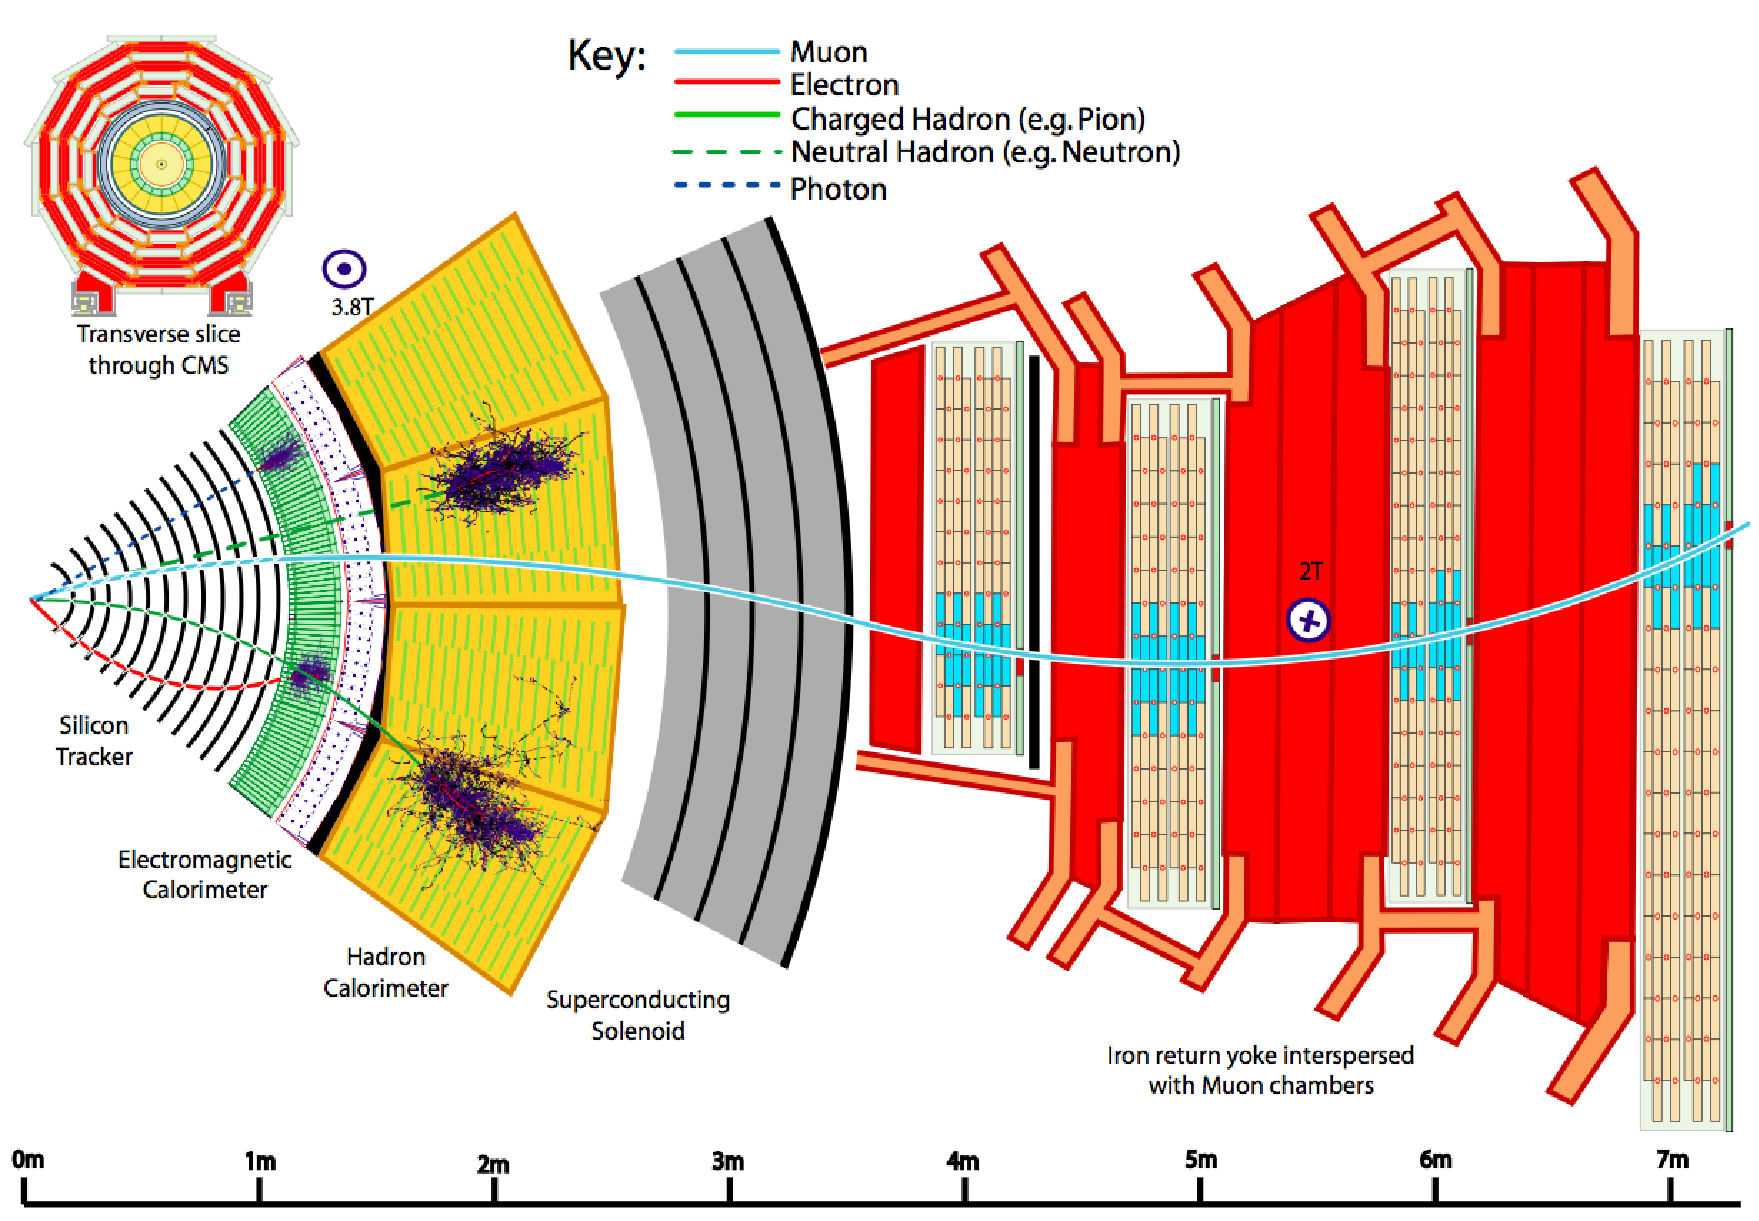
\includegraphics[width=0.95\textwidth]{detector/figs/CMS_Slice_2}
	\caption{A graphic depiction of different particles leaving various signatures in the different CMS detector subsystems. Particles may be detected via tracks hits, energy deposits, or a combination of both.}
	\label{fig:pfCandidates}
\end{figure}

\subsection{Isolation}
\label{subsec:iso}
Isolation is an important distinguishing variable for physics objects measured in the detector. Simply put, isolation measures the total amount of energy in some proximity to a physics object. Because many physics processes results in particle production outside the primary interaction vertex (such as showering, decays, hadronization, pair production, etc.), the isolation of a particle parametrizes the amount of other "activity" surrounding the physics object, and consequently proves a useful discriminant when determining if particles are produced in the primary interaction, or in subsequent physics processes. Particles which are produced in the primary physics process in a collision are sometimes referred to as {\it prompt}, and isolation is a powerful tool in identifying prompt leptons in particular.

\subsection{Electrons, Muons, and Photons}
\label{subsec:lepgamme}
The primary leptons considered in this analysis are electrons and muons (discussed in section \ref{subsec:muons}), and photons are also used as a cross-check in some control regions for background estimates. Prompt electrons and photons are identified in CMS primarily through the use of the ECAL, where they are stopped and deposit all their energy \cite{Baffioni:2006cd,Khachatryan:2015iwa}. Prompt electrons are customarily distinguished by both the presence of a track originating at the primary vertex and a sufficiently low isolation.

Electrons in CMS are identified primarily through the existence of a charged particle track terminating in an energy cluster in the ECAL. As described in section \ref{subsec:ecal}, the ECAL crystals are $\sim25$ radiation lengths deep, and will stop and contain nearly all of the energy of an electron (except perhaps minuscule losses to scattering in the tracker). The charged track leading to the energy deposit distinguishes the charged particle from a neutral particle, and the direction of curvature of the path in the tracker can be used to identify the charge of an electron (or positron).

Photons are distinguished from electrons by the lack of a track in the SVT. As a neutral particle, the only sign of a photon will be the energy deposit in the ECAL where the photon is stopped and deposits all its energy. Photons are typically distinguished from other neutral electromagnetic particles (such as a $\pi^0$) by the shape of the shower in the ecal. Whereas photons typically shower through pair production and bremsstrahlung, other hadronic particles may cascade via different physics processes leading to measurable difference in the shape of the energy cluster.

\subsection{Muons}
\label{subsec:muons}
Prompt muons produced in collisions at the LHC are generally minimum ionizing particles, and will penetrate the bulk of the detector. Without any matching calorimeter deposits, they are reconstructed using hits in the muon system matched to inner tracker hits \cite{Chatrchyan:2009ae}. The muon system flags muon candidates, which are then matched to inner tracker hits for the best fit of the muon track. Given the track hits, the transverse momentum and energy of the muon can be calculated by a fit to the track parameters. As with electrons, muons are customarily distinguished by both the presence of a track originating at the primary vertex and a sufficiently low isolation.

\subsection{Jets}
\label{subsec:jets}
Many particles produced at the LHC are created through the strong interaction, which may produce particles carrying color charge in the final state (i.e. quarks or gluons). Colored particles cannot exist individually due to the phenomenon known as {\it confinement}, and so via the process of {\it hadronization} (also refered to as {\it fragmentation}) they will proliferate in a series of interactions producing additional particle-antiparticle pairs, cascading in a parton shower to form hadronic bound states. When a "bare" quark or gluon is produced in the primary interaction, the ensuing hadronization results in a stream of tightly collimated hadrons aligned with the trajectory of the original bare particle, referred to as a {\it jet}. 

Jets present themselves in CMS as collimated energy deposits in both the ECAL and HCAL, as well as tracks originating at the primary vertex \cite{Schroder:2015czj}. Between the two calorimeters, all the electromagnetic and hadronic components of the jet are stopped and measured by the calorimeters, and any leptons (including muons detected in the muon system) which originate in the cone of the jet are assigned to the total jet energy. The jets are reconstructed using the "anti-k$_T$" algorithm, which clusters jet activity in cones of a fixed radius \cite{Cacciari:2008gp}. The jet is treated as a single physics object with a total energy equal to the sum of its electromagnetic, hadronic, and leptonic components, which by momentum conservation dictates the energy of the prompt quark or gluon that was produced in the primary interaction. 

Furthermore, the substructure of jets and their content can be analyzed to determine the flavor of the parent parton, known as "tagging". Jets are typically tagged to distinguish between those originating from heavy-flavor quarks (bottom or charmed) and light-flavor quarks. Top quarks produced in primary interactions are unique because of their short lifetime. A top quark will decay before hadronization occurs, instead producing a $W$ boson and down-type (down, bottom, or strange) quark which will subsequently hadronize. Searches involving top quarks in the final state typically employ "top-taggers" to search for these signatures of the top quark.

In practice, jets are complicated objects consisting of many constituent particles, and must be clustered and calibrated so that the jet energy closely matches that of the parent parton which produced the jet. Jet energy corrections (JECs) are applied to raw jet energies to compensate for different experimental deviations from the parent parton energy \cite{Khachatryan:2016kdb,CMS-DP-2016-020}. In particular, JECs include corrections to compensate for pileup energy as described in section \ref{subsec:pileup} \cite{Cacciari:2007fd}, detector effects (as a function of $\eta$), energy scale as a function of jet \pt, and residual corrections to account for differences between data and simulation. The JECs are calculated by collecting data events with a Z boson (decaying to electrons or muons) or photon recoiling against a jet. By precisely measuring the bosons energy with the ECAL, scale factors are derived for jets as a function of pseudorapidity $\eta$ and momentum \pt. 

\subsection{Missing Energy}
\label{subsec:met}
Missing energy refers to the sum of all energy which has escaped the detector, and is inferred from a momentum-imbalance in the physics objects measured by the detector \cite{Chatrchyan:2011tn}. Because the momentum of the incident protons is zero perpendicular to the direction of the beam, the momentum of physics objects produced in any collision must sum to zero in the direction transverse to the beamline. The missing transverse energy (\MET), is calculated by taking the negative vector sum of all PF candidates as in equation \ref{eq:met}. \MET is of particular importance to analyses targeting BSM physics, as BSM signatures characteristically contain invisible particles in the final state which escape detection.
\begin{equation}
	\label{eq:met}
	\vec{E}_T^{miss}=-\sum_i^{} \vec{p}_T^{\: i}
\end{equation}

The missing energy in an event is inferred from all other measured quantities in an event, and there are many sources of \MET which are unphysical in nature but rather dependent on experimental effects. Particles from the primary interaction with a sufficiently large pseudorapidity may escape the fiducial region of the detector subsystems, and resolution effects or intrinsic noise in the detector may lead to fluctuations in measured energies. These experimental effects must be suppressed or distinguished from "real" \MET due to physics processes creating particles which escape the detector (e.g. neutrinos). Analyses sensitive to final states with \MET often employ robust data-driven methods to predict or suppress backgrounds which might generate experimental sources of \MET or physics processes which can contribute real \MET (such as \znunu).

% --------------------------------------------------------------------------- %
% --------------------------------------------------------------------------- %
